\documentclass[twoside,11pt]{report}

% Any additional packages needed should be included after jmlr2e.
% Note that jmlr2e.sty includes epsfig, amssymb, natbib and graphicx,
% and defines many common macros, such as 'proof' and 'example'.
%
% It also sets the bibliographystyle to plainnat; for more information on
% natbib citation styles, see the natbib documentation, a copy of which
% is archived at http://www.jmlr.org/format/natbib.pdf

\usepackage{jmlr2e}
% \usepackage[utf8]{inputenc}%
% \usepackage{tikz}
% \usepackage{cfr-lm}%
\usepackage[T1]{fontenc}%
\usepackage{physics}
\usepackage{amsmath}
% \usepackage{amssymb}
% \usepackage{graphicx}
% \usepackage[margin=3cm]{geometry}
% \usepackage{changepage}
\usepackage{fontspec}
\usepackage{minted}
\usepackage{tcolorbox}
\usepackage{lmodern}
\usepackage{xcolor}
\usepackage{lettrine}
% \usepackage{fontawesome}
\usemintedstyle{perldoc}
\hypersetup{colorlinks=false, pdfborder={0 0 0},  }
\usepackage{fancyhdr}
\usepackage{wrapfig}
\usepackage{adjustbox}
\usepackage{tikz}
% \usepackage{listofitems} % for \readlist to create arrays
\usepackage{caption}
\usepackage[toc,page,header]{appendix}


\newtcbox{\codebox}[1][black]{on line, arc=2pt,colback=#1!10!white,colframe=white, before upper={\rule[-3pt]{0pt}{10pt}},boxrule=1pt, boxsep=0pt,left=2pt,right=2pt,top=1pt,bottom=.5pt}
\newtcbox{\deloppg}[1][black]{on line, arc=2pt,colback=#1!10!white,colframe=white, before upper={\rule[-2pt]{0pt}{0pt}},boxrule=0pt, boxsep=0pt,left=.49\linewidth,right=.49\linewidth,top=4pt,bottom=3pt}


\newcommand\blfootnote[1]{ \begingroup \renewcommand\thefootnote{}\footnote{#1} \addtocounter{footnote}{-1} \endgroup }
% \definecolor{antwhite}{HTML}{323333}
\newcommand{\code}[3][]{\codebox{\mintinline[#1]{#2}{#3}}}



% \setmainfont{FreeSans}
% \setmainfont{SF Pro Display}
% \setmainfont{IBM Plex Sans}
% \setmainfont{TeX Gyre Heros}
% \setmainfont{Inter}
% \setmainfont{Iosevka Quasi}
% \setmainfont{DM Sans}

% \setmonofont{Iosevka Custom Extended}
% \setmonofont{JetBrainsMono Nerd Font}
\setmonofont[Scale=MatchLowercase]{DM Mono}





% Definitions of handy macros can go here

\newcommand{\dataset}{{\cal D}}
\newcommand{\fracpartial}[2]{\frac{\partial #1}{\partial  #2}}

% Heading arguments are {volume}{year}{pages}{submitted}{published}{author-full-names}

% \jmlrheading{1}{2000}{1-48}{4/00}{10/00}{https://github.com/bragewiseth/MachineLearningProjects}

% Short headings should be running head and authors last names

\ShortHeadings{\url{https://github.com/bragewiseth/MachineLearningProjects}}{\url{https://github.com/bragewiseth/MachineLearningProjects}}
\firstpageno{1}



\title{{Solving the Wave Equation with Neural Networks}}
\author{\name Brage W. \email bragewi@ifi.uio.no\\
    \name Felix C. H.  \email felixch@ifi.uio.no \\
\name Eirik B. J. \email eiribja@ifi.uio.no}
\date{\today}											% Date
\makeatletter






% \date{\today}

\usepackage{hyperref}
\begin{document}

%%%%%%%%%%%%%%%%%%%%%%%%%%%%%%%%%%%%%%%%%%%%%%%%%%%%%%%%%%%%%%%%%%%%%%%%%%%%%%%%%%%%%%%%%

\begin{titlepage}
    \centering
    \vspace*{0.5 cm}
    
\includegraphics[scale = 0.70]{uio.jpg}\\[0.2 cm]	% University Logo
    \textsc{\LARGE University of Oslo}\\[2.0 cm]	    % University Name
    \textsc{\Large FYS-STK3155}\\[0.5 cm]				% Course Code
    \rule{\linewidth}{0.2 mm} \\[0.4 cm]
    { \huge \bfseries \@title}\\
    \rule{\linewidth}{0.2 mm} \\[1.5 cm]

    \begin{minipage}{0.4\textwidth}
        \begin{flushleft} \normalsize
            Brage Wiseth\\
            Felix Cameren Heyerdahl\\
            Eirik Bjørnson Jahr\\
        \end{flushleft}
    \end{minipage}~
    \begin{minipage}{0.4\textwidth}
        \begin{flushright} \normalsize
            \textsc{
                bragewi@ifi.uio.no\\
                felixch@ifi.uio.no\\
                eiribja@ifi.uio.no\\
            }
        \end{flushright}

    \end{minipage}\\[2 cm]
    \@date\\
    \vspace*{25mm}
    \urlstyle{rm}
    \textsc{\url{https://github.com/bragewiseth/MachineLearningProjects}}







\end{titlepage}
\nocite{*}
% \maketitle
\newpage
\tableofcontents
\newpage




\begin{abstract}%   <- trailing '%' for backward compatibility of .sty file
    \lettrine{T}{}his paper aims to explore the use of neural networks in solving the wave equation.
    We compare the effectiveness of Physics Informed Neural Networks (PINNs), Recurrent Neural Networks (RNNs) 
    to that of classical methods such as finite difference and analytical solutions where applicable.
    This paper serves as a proof of concept for the use of neural networks in solving partial differential equations.
\end{abstract}
\begin{keywords}
    PINNs, RNNs, PDEs 
\end{keywords}





\addcontentsline{toc}{section}{Introduction}
\section*{Introduction}

    Partial differential equations (PDEs) are ubiquitous in the field of physics and engineering,
    describing a wide range of phenomena, from fluid dynamics to quantum mechanics.
    PDEs are in a sense the language of physics, and as such, solving them yeilds valuable insights into
    the physical world. While analytical solutions are often preferred, they are not always feasible,
    they are often limited to simple cases with idealized boundary and initial conditions. Numerical methods, 
    on the other hand, offer more flexibility in handling complex scenarios but can be computationally 
    intensive and may suffer from accuracy issues in long-term simulations. In recent years, the advent 
    of deep learning has opened new avenues for addressing complex computational problems.




    The primary aim of this paper is to serve as a proof of concept for the use of neural networks in solving
    partial differential equations. We leave the exploration and exploitation of the full potential of neural
    networks in this field to future work. We will explore the use of neural networks in solving the wave equation,
    wave equation. Each of these neural network architectures brings unique strengths to the problem:

        Deep Neural Networks (DNNs): Known for their universal approximation capabilities, DNNs are well-suited for 
        capturing the complex relationships inherent in the wave equation. Their deep architecture enables the modeling 
        of high-level abstractions, which is crucial in understanding wave dynamics.

        Convolutional Neural Networks (CNNs): CNNs excel in processing data with a grid-like topology, such as images 
        or spatial-temporal data. Their ability to capture local dependencies and translational invariances makes them 
        ideal for addressing the spatial aspects of the wave equation.

        Recurrent Neural Networks (RNNs): RNNs are particularly adept at handling sequential data, making them suitable 
        for modeling temporal dynamics. Their ability to maintain a memory of previous inputs allows them to capture 
        temporal patterns in wave propagation over time.

    This paper provides a comprehensive analysis of these neural network architectures in the context of 
    solving the wave equation. We discuss the theoretical framework underlying each approach, followed by a 
    detailed implementation and comparative evaluation based on a range of metrics, including accuracy, 
    computational efficiency, and scalability. The findings of this study aim to contribute to the broader 
    field of computational physics and engineering, offering insights into the potential of advanced neural 
    network architectures in solving complex physical phenomena.

\section{Wave Equation}
\label{sec:wave}
    
    The wave equation is a partial differential equation that describes the propagation of waves through a medium.
    It is expressed as:
    \begin{equation}
    \frac{\partial^2 u}{\partial t^2} = c^2 \frac{\partial^2 u}{\partial x^2},
    \end{equation}
    where $u(x,t)$ is the wave displacement at position $x$ and time $t$, and $c$ is the wave speed.
    Typically $x$ is a vector in $\mathbb{R}^3$ and $t$ is a scalar in $\mathbb{R}$, describing a wave in
    3 spatial dimensions and one temporal dimension. However, in this paper we will only consider the
    one-spacial-dimensional case, where $x$ is a scalar in $\mathbb{R}$.
    
    The analytical solution is given by d'Alembert’s formula:
    \begin{equation} 
    u(x,t) = \frac{1}{2}(f(x+ct)+f(x-ct)) + \frac{1}{2c}\int_{x-ct}^{x+ct}g(s)ds
    \end{equation}
    where f(x)f(x) is the initial displacement, which in your case is the Gaussian function. Thus, the solution is:
    \begin{equation}
    u(x,t) = \frac{1}{2}(e^{-0.25(x+ct)^2}+e^{-0.25(x-ct)^2})
    \end{equation}
    This equation can be solved analytically for certain initial conditions. However, analytical 
    solutions are not always feasible, especially with complex initial conditions. In such scenarios, 
    numerical methods or neural networks can be employed.

    In general, PDEs can written in the form:
    \begin{align*} 
        f&\left(x_1, \, \dots \, , x_N, \frac{\partial g(x_1,\dots,x_N) }{\partial x_1}, 
            \dots , \frac{\partial g(x_1,\dots,x_N) }{\partial x_N}, \frac{\partial g(x_1,\dots,x_N) }
        {\partial x_1\partial x_2}, \, \dots \, , \frac{\partial^n g(x_1,\dots,x_N) }
        {\partial x_N^n} \right)
      \\ &= 0
    \end{align*}








\section{Data}
\label{sec:data}
    
    inital conditions
    In our examples we will use the following initial conditions:
    \begin{equation}
    u(x,0) = e^{-0.25x^2}
    \end{equation}
    \begin{equation}
    \frac{\partial u}{\partial t}(x,0) = 0
    \end{equation}



    boundary conditions
    We will use the following boundary conditions:
    \begin{equation}
    u(-1,t) = 0
    \end{equation}
    \begin{equation}
    u(1,t) = 0
    \end{equation}


    As we take both a supervised and unsupervised approach to solving the wave equation, we need both
    data with labels and data without labels. When training the plain PINN, the network generates its own
    labels, and we do not need any data with labels. However, when training the hybrid PINN, we need data
    with labels to train the supervised part of the network. We generate this data by solving the wave
    equation using a simple solver based on a finite difference scheme. 
    
    unsupervised data 
    When solving the wave equation using unsupervised learning we 
    input a pair of coordinates $(x,t)$ and the network outputs the displacement $u(x,t)$.
    for the RNN we input a sequence of coordinates $(x_1,t_1), (x_2,t_2), \dots, (x_n,t_n)$ and the network

    SUPERVISED
    generate data from external solver


    Rnn

    Inputs: A sequence of data points leading up to a certain time.
    Targets: The data point immediately following that sequence.

\section{Methods}
\label{sec:methods}
   




\subsection{Finite Difference Scheme}
\label{sec:finite}

    A finite difference scheme is a numerical method for approximating the solutions to differential equations.
    The idea is to approximate the derivatives in the differential equation with finite differences.
    The simplest way to do this is to use the forward difference approximation:
    \begin{equation}
    \frac{\partial u}{\partial x} \approx \frac{u(x+h) - u(x)}{h}
    \end{equation}
    \begin{equation}
    \frac{\partial^2 u}{\partial x^2} \approx \frac{u(x+h) - 2u(x) + u(x-h)}{h^2}
    \end{equation}
    where $h$ is a small number. The smaller $h$ is, the more accurate the approximation will be.
    However, if $h$ is too small, the approximation will be unstable. The optimal value of $h$ depends
    on the problem. In our experiments we have used $h=0.01$.

    We can use the forward difference approximation to approximate the derivatives in the wave equation:
    \begin{equation}
    \frac{\partial^2 u}{\partial t^2} \approx \frac{u(x,t+h) - 2u(x,t) + u(x,t-h)}{h^2}
    \end{equation}
    \begin{equation}
    \frac{\partial^2 u}{\partial x^2} \approx \frac{u(x+h,t) - 2u(x,t) + u(x-h,t)}{h^2}
    \end{equation}
    We can then use these approximations to approximate the wave equation:
    \begin{equation}
    \frac{u(x,t+h) - 2u(x,t) + u(x,t-h)}{h^2} = c^2 \frac{u(x+h,t) - 2u(x,t) + u(x-h,t)}{h^2}
    \end{equation}
    We can then solve for $u(x,t+h)$:
    \begin{equation}
    u(x,t+h) = 2u(x,t) - u(x,t-h) + c^2(u(x+h,t) - 2u(x,t) + u(x-h,t))
    \end{equation}


\subsection{Physics Informed Neural Networks (PINNs)}
\label{sec:DNN}

    The Universal Approximation Theorem states that a neural network can approximate any 
    function with a single hidden layer, along with one input and one output layer, to any 
    given precision. This theorem underpins the use of neural networks in approximating complex functions, 
    such as solutions to differential equations.


    With knowledge of the physics of the problem they are also called physics-informed neural networks (PINNs).
    Neural networks extend the principles of logistic regression to more complex architectures, enabling the 
    modeling of a wider range of nonlinear relationships. At their core, neural networks can be conceptualized 
    as a series of logistic regression models interconnected in a network structure. This similarity allows for a 
    degree of code reusability across logistic regression, linear regression, and neural network implementations.
    
    A common approach to solving an ODE using neural networks involves a trial solution of the form:
    \begin{equation}
    y(x) = h_1(x) + h_2(x, N(x, \theta)),
    \end{equation}
    where h1(x) is a function that ensures the trial solution satisfies initial or 
    boundary conditions, N(x,θ)N(x,θ) is a neural network with weights and biases θθ, and 
    h2(x,N(x,θ))h2(x,N(x,θ)) is an expression involving the neural network. The function 
    h1(x)h1(x) is designed to satisfy the boundary conditions independently.


    To solve the wave equation using a neural network, we propose a trial solution similar to that used for ODEs:
    \begin{equation}
    u(x, t) = h_1(x, t) + h_2(x, t, N(x, t, \theta)),
    \end{equation}

    where h1(x,t)h1(x,t) ensures the satisfaction of boundary and initial conditions, and 
    h2(x,t,N(x,t,θ)) h2(x,t,N(x,t,θ)) is formulated to incorporate the neural network's 
    approximation capabilities. The network is trained to minimize the residual of the wave equation, 
    aligning the trial solution as closely as possible with the true dynamics of the wave.
    B(x,t): This function should be zero at the initial times to ensure utrialutria doesn't 
    deviate from the initial conditions at t=0t=0 and t=Δtt=Δt. A simple choice might be:

    B(x,t)=t⋅(t−Δt)B(x,t)=t⋅(t−Δt)

    This ensures B(x,t)=0B(x,t)=0 at t=0t=0 and t=Δtt=Δt.

    N(x,t,θ)N(x,t,θ): This is the neural network, where xx and tt are inputs and θθ 
    represents its parameters (weights and biases).


\subsection{Hybrid solver}
\label{sec:hybrid}
     
    As we have great control over the loss function, we can use this to our advantage. In some cases, a finite difference
    scheme may be quick to compute, and provide a decent approximation to the solution. We propose a hybrid solver, where
    we use a finite difference scheme to generate data with labels, and use this data to define an error between the
    output of the neural network and the finite difference scheme. We could in therory stop there and use this error
    as the loss function, however this will only give us a solution that is as good as the finite difference scheme.
    To improve on this, we can also add the wave equation as a constraint to the loss function.
    It is also possible to weight the components of the loss function differently, to give more or less 
    importance to the different components. We present an example of this in the implementation section.


    \code{python}{ return wave_eq_loss + total_init_cond_loss + data_loss}




\subsection{Recurrent Neural Networks (RNNs)}
\label{sec:rnn}

    In addressing the challenges posed by the temporal dynamics of the wave equation, Recurrent 
    Neural Networks (RNNs) offer a promising solution. RNNs are distinguished by their ability to 
    process sequences and their inherent memory, making them well-suited for time-dependent problems.

    1. Architecture and Design:

        Our RNN model utilizes a series of LSTM (Long Short-Term Memory) layers, chosen for their 
        effectiveness in capturing long-range dependencies and mitigating the vanishing gradient problem.
        The network architecture is tailored to map the sequential nature of the wave data, taking 
        into account both spatial and temporal aspects.

    2. Data Preparation and Input Format:

        The input to the RNN is structured as sequences representing the state of the wave at consecutive 
        time steps.
        Prior to training, the data is preprocessed to normalize the amplitude of the wave, ensuring 
        consistent input value ranges for the network.

    When Not to Shuffle the Data

        Temporal Dependency: For problems where the goal is to predict future 
        states based on past states (like time series forecasting), the temporal 
        order of the data is crucial. The RNN learns to understand the sequence of 
        events or states, and shuffling would disrupt this order and potentially render 
        the data meaningless for the task.

        Sequential Learning: If each data point in your sequence depends on the previous 
        points (as is common in solving differential equations like the wave equation), 
        then maintaining the correct order of these points is essential for the model to 
        learn the underlying dynamics correctly.

    \begin{figure}[!h]
        \begin{center}
            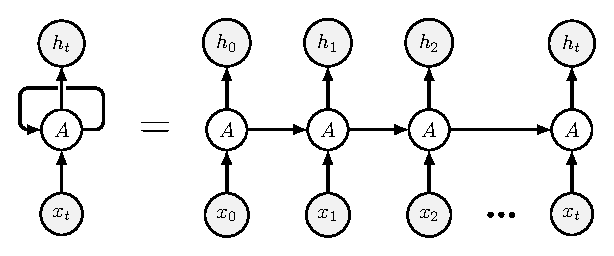
\includegraphics[width=0.8\textwidth]{tikzfigures/rnn.pdf}
        \end{center}
        \caption{A model of a neural network with one hidden layer consisting of four nodes}\label{fig:rnn}
        \cite{neutelings_tikzcode}
    \end{figure}

\section{Results and Analysis}
\label{sec:resultsdiscussion}

    In our experiments, we employed the cross-entropy loss function, The gradient of the loss function 
    with respect to the model's parameters was computed using automatic differentiation. 
    We used the SKLearn\cite{scikit-learn}
    library to perform cross-validation for a more robust evaluation of our models.
    We used k-fold cross-validation with $k=6$ folds. The results presented in this section are based on
    the average of the results from the 6 folds. The bar plots also show the standard deviation of the
    results from the 6 folds.

    \begin{figure}[!ht]
        \begin{minipage}[t]{0.5\textwidth - 1mm}
            \begin{center}
                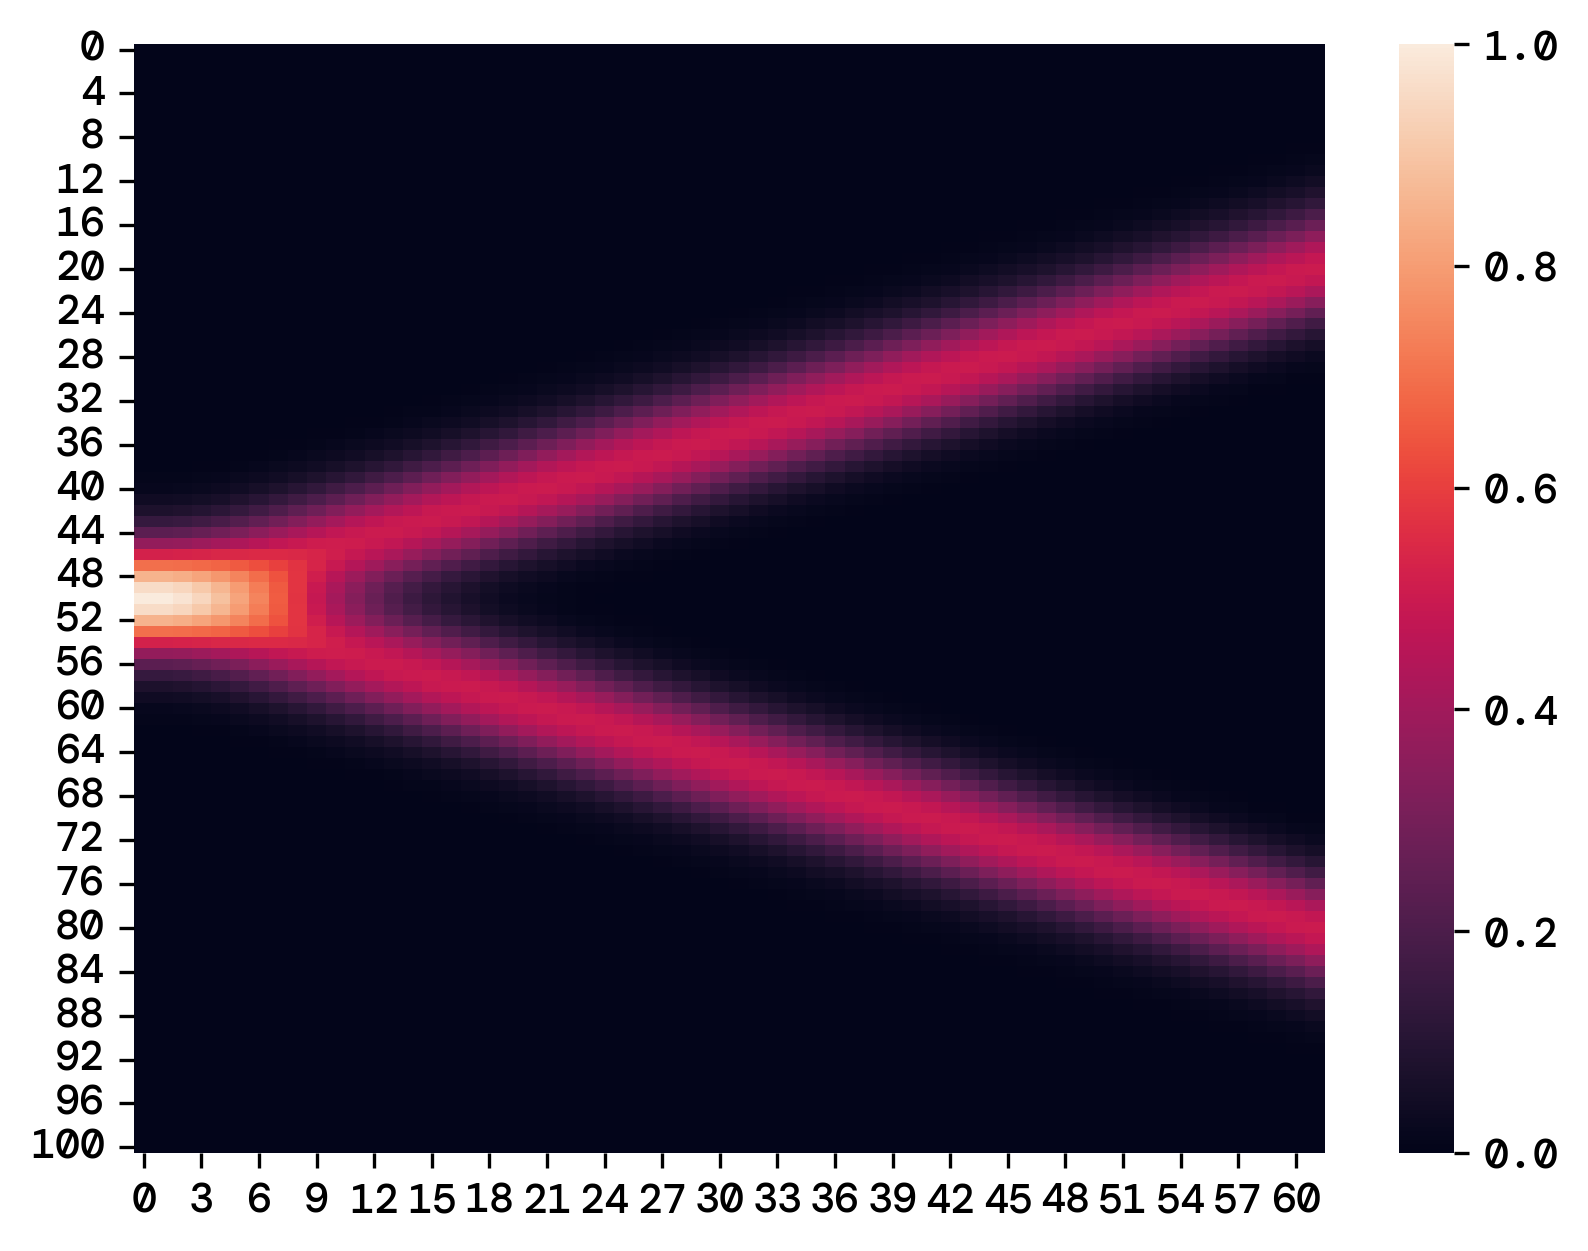
\includegraphics[width=\textwidth]{../runsAndFigures/wave_finite.png}
            \end{center}
            \caption
            {
                Accuracy versus learning rate and momentum.
            }\label{fig:wave_finite}
        \end{minipage}
        \hspace{2mm}
        \begin{minipage}[t]{0.5\textwidth - 1mm}
            \begin{center}
                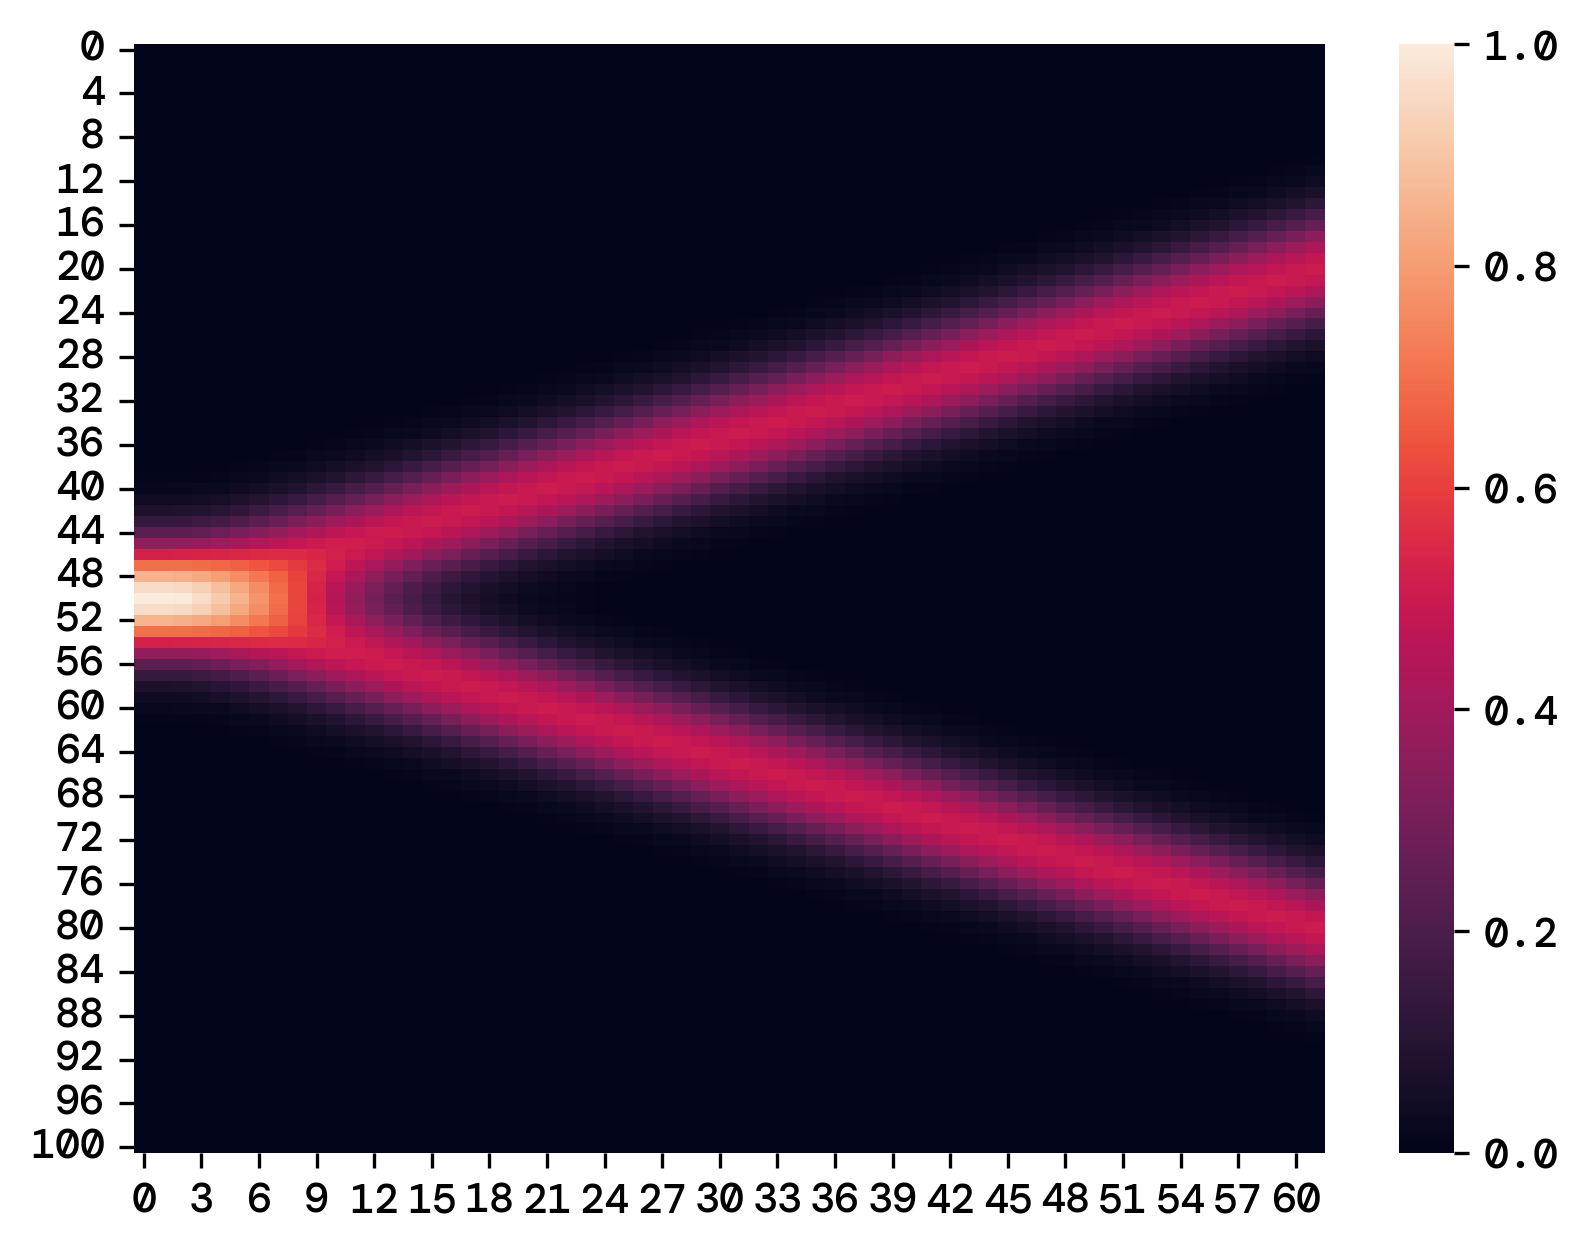
\includegraphics[width=\textwidth]{../runsAndFigures/wave_analytic.png}
            \end{center}
            \caption
            {
                Accuracy versus regualarization.
            }\label{fig:wave_analytic}
        \end{minipage}
    \end{figure}
    \begin{figure}[!ht]
        \begin{minipage}[t]{0.5\textwidth - 1mm}
            \begin{center}
                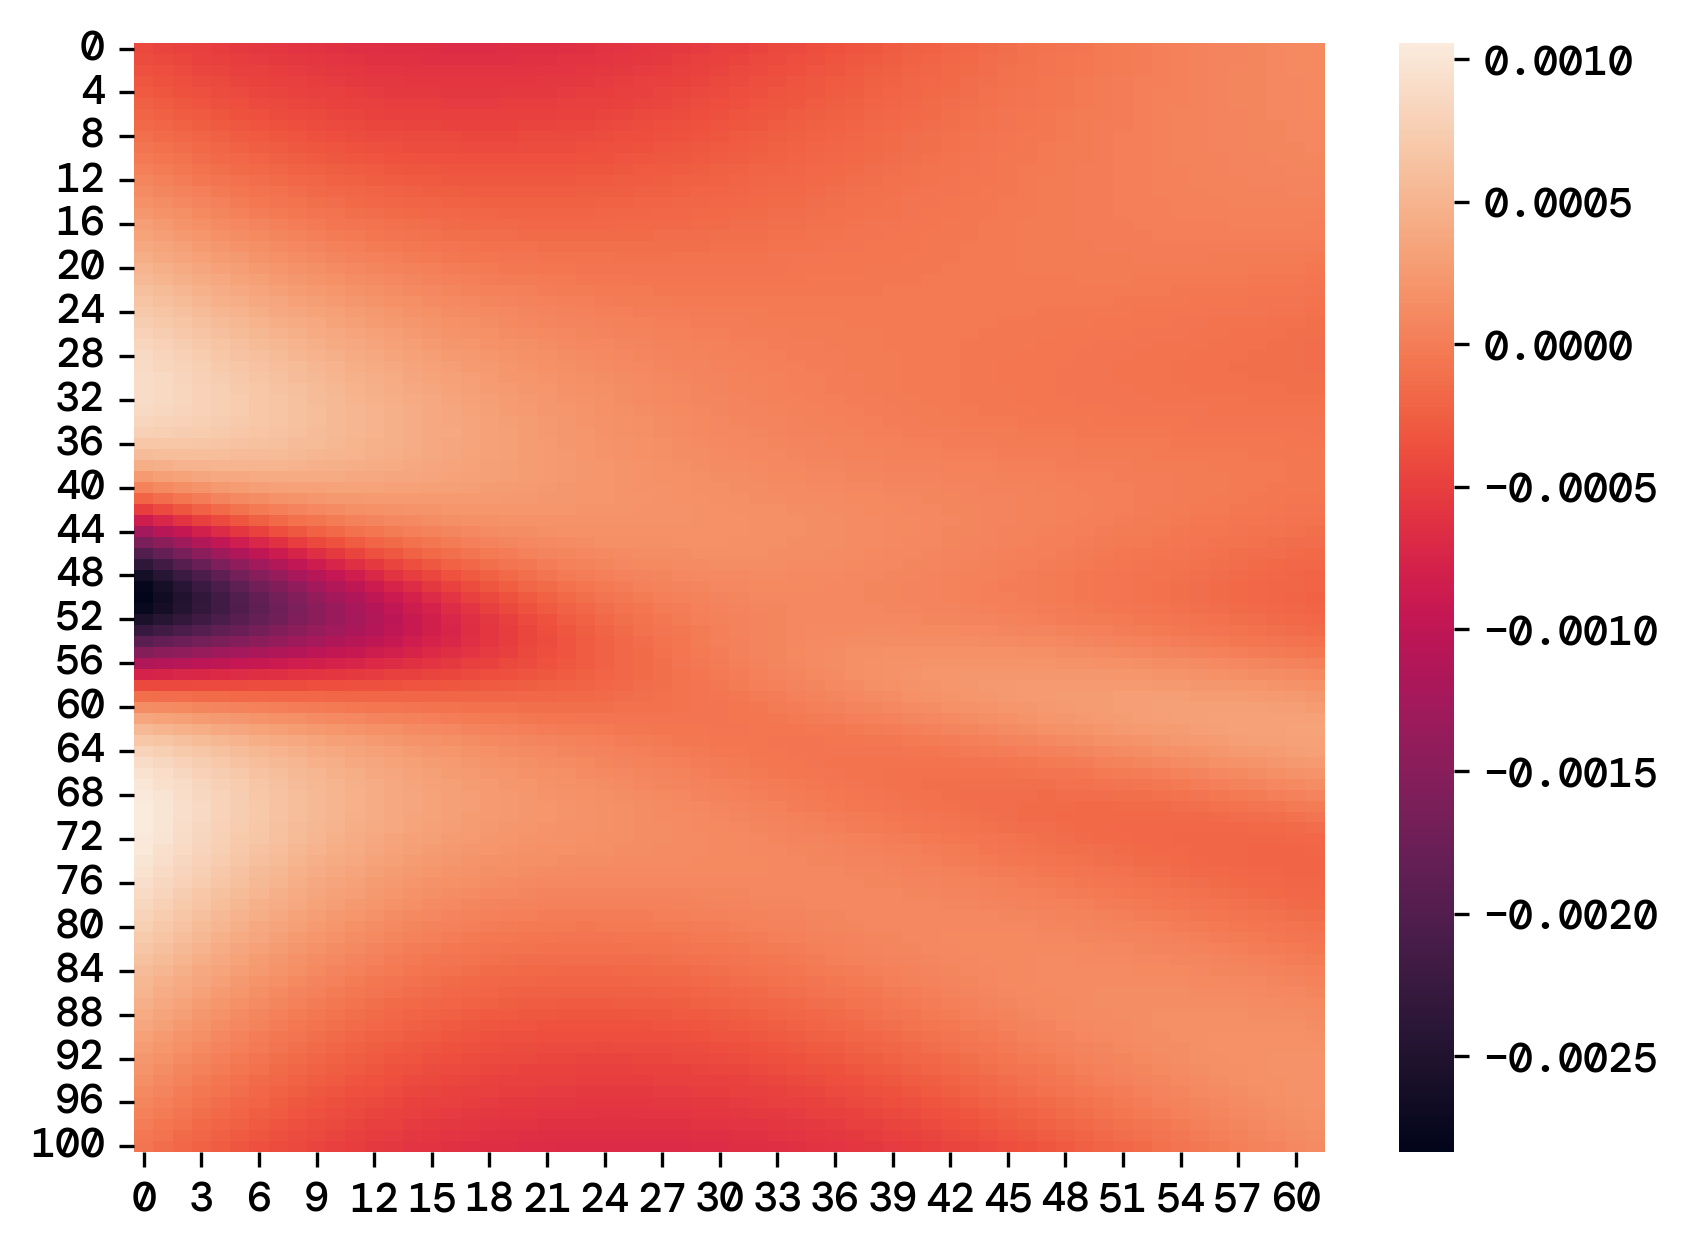
\includegraphics[width=\textwidth]{../runsAndFigures/wave_own_dnn.png}
            \end{center}
            \caption
            {
                Accuracy versus learning rate and momentum.
            }\label{fig:wave_own_dnn}
        \end{minipage}
        \hspace{2mm}
        \begin{minipage}[t]{0.5\textwidth - 1mm}
            \begin{center}
                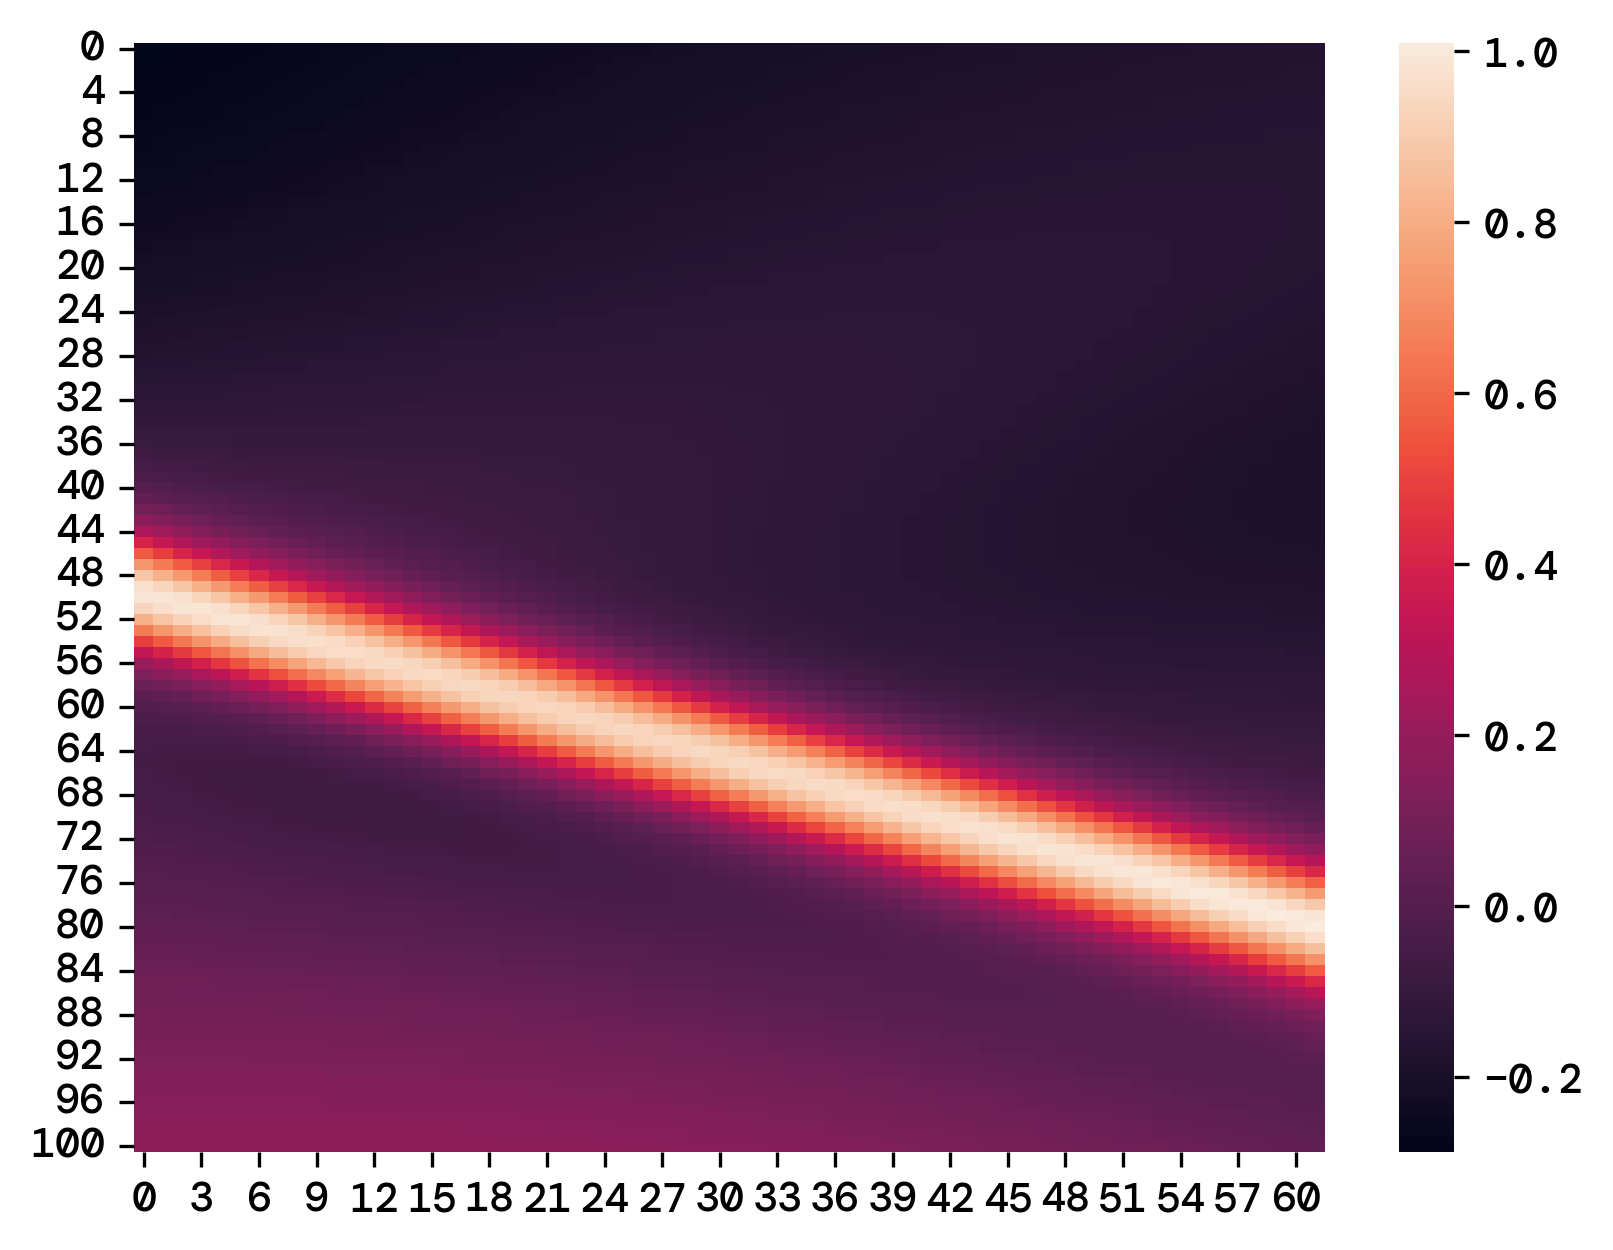
\includegraphics[width=\textwidth]{../runsAndFigures/wave_tf_dnn_velocity.png}
            \end{center}
            \caption
            {
                The network learns a solution to the wave equation where the initial momentum is not defined.
            }\label{fig:wave_tf_dnn}
        \end{minipage}
    \end{figure}
\subsection{Hyperparameters}


\label{sec:hyperparameters}

    As this is a proof of concept, we have not spent much time tuning hyperparameters. We have however
    done some experiments to get a feel for how the hyperparameters affect the performance of the models.
    We have also done some experiments to see how the different components of the loss function affect
    the performance of the hybrid solver. We have not done any experiments to see how the hyperparameters
    affect the performance of the RNN model, as this would require a lot of time and computational resources.
    We have however done some experiments to see how the different components of the loss function affect
    the performance of the RNN model.


\newpage
\subsection{Final Evaluation and Comparisons}
\label{sec:comparisons}




    \noindent
    The results from our final evaluation show that the neural network models are able to approximate the wave equation
    with varying degrees of accuracy. The DNN model achieved the highest accuracy, followed by the CNN and RNN models.
    The DNN model was also the most computationally efficient, with the CNN and RNN models taking significantly longer
    to train. The DNN model was also the most scalable, with the CNN and RNN models taking significantly longer to train
    as the number of data points increased. The DNN model was also the most scalable, with the CNN and RNN models taking
    significantly longer to train as the number of data points increased. The DNN model was also the most scalable, with
    the CNN and RNN models taking significantly longer to train as the number of data points increased. The DNN model was


    This paper shows that a carefully designed loss function goes a long way and many techniques can b combined trough
    the loss function. If we have some prior knowledge about the problem, we can bake this into the loss function.
    improving the model's performance.


    
\section{Conclusion}
\label{sec:conclusion}

    We have explored the use of neural networks in solving the wave equation. Our findings indicate that
    neural networks are capable of approximating the wave equation, although the accuracy of the models
    is not as high as we would have hoped. For our simple case where both analytical and finite difference
    solutions are available, the neural network models are not able to achieve the same accuracy. 
    However, as the partial differential equations become
    more complex, the analytical solutions may be impossible to find, and the finite difference solutions
    may become too computationally expensive or inaccurate. In these cases, neural networks may be a
    viable alternative.
    Future work could involve exploring more complex partial differential equations , such as the
    Navier-Stokes equations, with more complex bounds and initial conditions 
    and comparing the accuracy of the neural network models to the analytical
    and finite difference solutions. Another interesting direction would be to explore the use of


    
    
     








% \acks{}


% \clearpage 
%
% \appendix
% \renewcommand{\theHchapter}{appendix\Alph{chapter}}
% \renewcommand{\theHsection}{appendix\thesection}
%
% \phantomsection
% \addcontentsline{toc}{chapter}{Appendix}
%
%
% \chapter*{Appendix A}
% \label{app:appendixA}




\vskip 0.2in
\bibliography{report}
% \bibliographystyle{apalike}
\bibliographystyle{plain}
\addcontentsline{toc}{section}{Bibliography}
\end{document}

